\documentclass{standalone}
\usepackage{tikz}
\usetikzlibrary{patterns, positioning}
\usepackage[sfdefault]{ClearSans} %% option 'sfdefault' activates Clear Sans as the default text font
\usepackage[T1]{fontenc}

\begin{document}
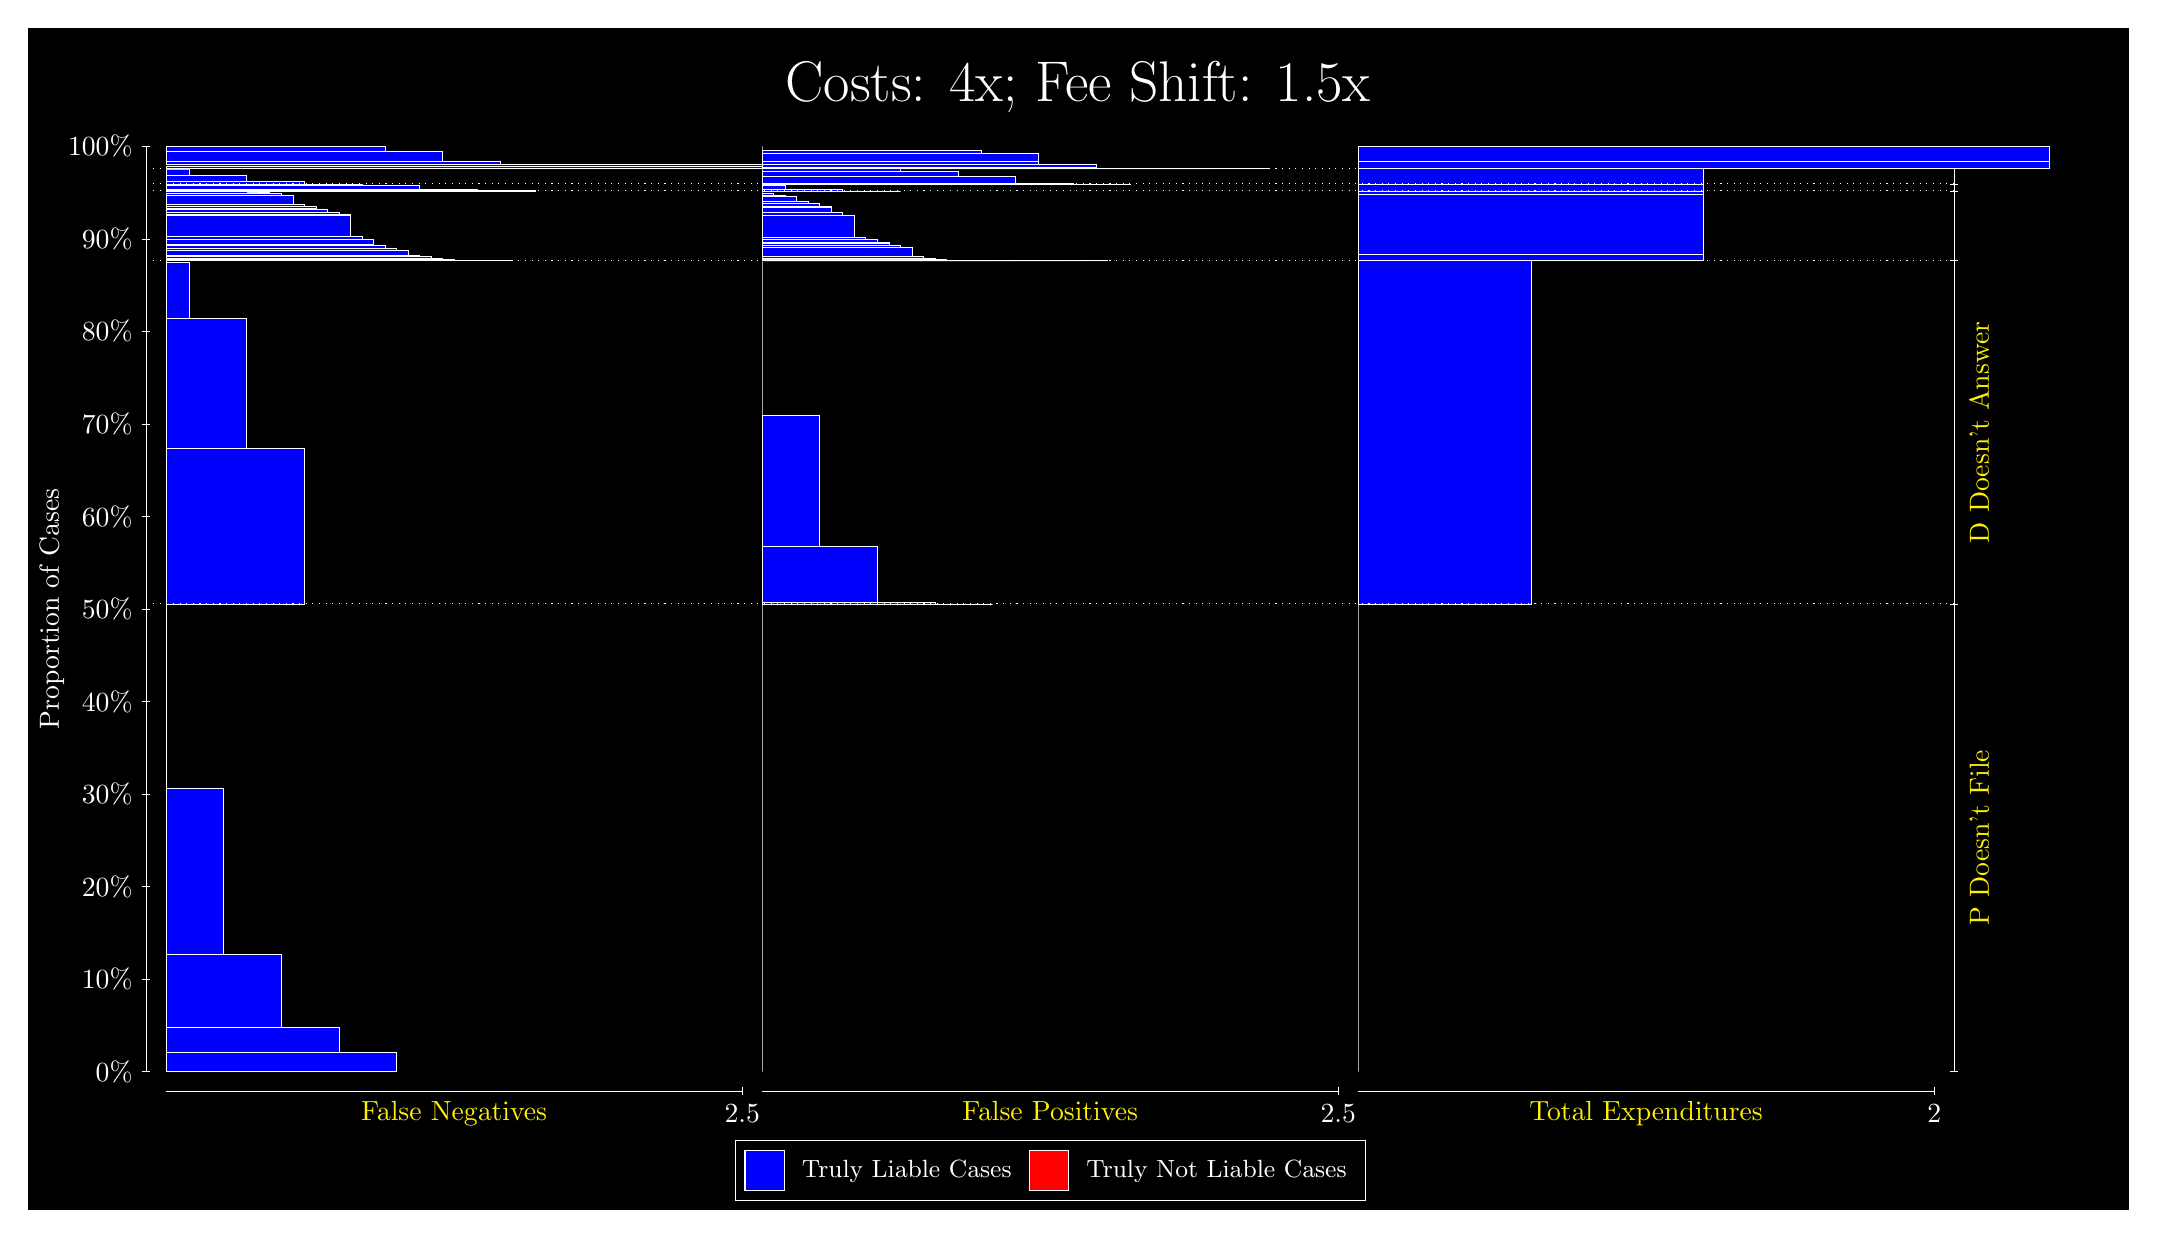
\begin{tikzpicture}
\draw[fill=black] (0,0) rectangle (26.667,15);
\draw[text=white] (0,13.5) rectangle (26.667,15) node[midway] {\huge Costs: 4x; Fee Shift: 1.5x};
\draw[white, very thin] (1.5,1.75) -- (1.5,13.5);
\node[rotate=90, text=white, anchor=center] at (0.3, 7.625) {Proportion of Cases};
\draw[white, very thin] (1.45,1.75) -- (1.55,1.75);
\node[text=white, anchor=east] at (1.45, 1.75) {0\%};
\draw[white, very thin] (1.45,2.925) -- (1.55,2.925);
\node[text=white, anchor=east] at (1.45, 2.925) {10\%};
\draw[white, very thin] (1.45,4.1) -- (1.55,4.1);
\node[text=white, anchor=east] at (1.45, 4.1) {20\%};
\draw[white, very thin] (1.45,5.275) -- (1.55,5.275);
\node[text=white, anchor=east] at (1.45, 5.275) {30\%};
\draw[white, very thin] (1.45,6.45) -- (1.55,6.45);
\node[text=white, anchor=east] at (1.45, 6.45) {40\%};
\draw[white, very thin] (1.45,7.625) -- (1.55,7.625);
\node[text=white, anchor=east] at (1.45, 7.625) {50\%};
\draw[white, very thin] (1.45,8.8) -- (1.55,8.8);
\node[text=white, anchor=east] at (1.45, 8.8) {60\%};
\draw[white, very thin] (1.45,9.975) -- (1.55,9.975);
\node[text=white, anchor=east] at (1.45, 9.975) {70\%};
\draw[white, very thin] (1.45,11.15) -- (1.55,11.15);
\node[text=white, anchor=east] at (1.45, 11.15) {80\%};
\draw[white, very thin] (1.45,12.325) -- (1.55,12.325);
\node[text=white, anchor=east] at (1.45, 12.325) {90\%};
\draw[white, very thin] (1.45,13.5) -- (1.55,13.5);
\node[text=white, anchor=east] at (1.45, 13.5) {100\%};

\draw[white, very thin] (24.457,1.75) -- (24.457,13.5);
\draw[white, very thin] (24.407,1.75) -- (24.507,1.75);
\node[anchor=west] at (24.407, 1.75) {};
\draw[white, very thin] (24.407,7.6888) -- (24.507,7.6888);
\node[anchor=west] at (24.407, 7.6888) {};
\draw[white, very thin] (24.407,12.049) -- (24.507,12.049);
\node[anchor=west] at (24.407, 12.049) {};
\draw[white, very thin] (24.407,12.934) -- (24.507,12.934);
\node[anchor=west] at (24.407, 12.934) {};
\draw[white, very thin] (24.407,13.024) -- (24.507,13.024);
\node[anchor=west] at (24.407, 13.024) {};
\draw[white, very thin] (24.407,13.218) -- (24.507,13.218);
\node[anchor=west] at (24.407, 13.218) {};
\draw[white, very thin] (24.407,13.5) -- (24.507,13.5);
\node[anchor=west] at (24.407, 13.5) {};

\draw[white, very thin, fill=blue] (1.75,1.75) rectangle (4.6775,1.9913);
\draw[white, very thin, fill=blue] (1.75,1.9913) rectangle (3.9457,2.3162);
\draw[white, very thin, fill=blue] (1.75,2.3162) rectangle (3.2138,3.2449);
\draw[white, very thin, fill=blue] (1.75,3.2449) rectangle (2.4819,5.3414);
\draw[white, very thin, fill=red] (1.75,5.3414) rectangle (1.75,5.3414);
\draw[white, very thin, fill=blue] (1.75,5.3414) rectangle (1.75,7.6888);
\draw[white, very thin, fill=blue] (1.75,7.6888) rectangle (3.5065,9.6599);
\draw[white, very thin, fill=blue] (1.75,9.6599) rectangle (2.7746,11.313);
\draw[white, very thin, fill=blue] (1.75,11.313) rectangle (2.0428,12.027);
\draw[white, very thin, fill=red] (1.75,12.027) rectangle (1.75,12.027);
\draw[white, very thin, fill=blue] (1.75,12.027) rectangle (1.75,12.049);
\draw[white, very thin, fill=blue] (1.75,12.049) rectangle (6.1413,12.05);
\draw[white, very thin, fill=blue] (1.75,12.05) rectangle (5.8486,12.053);
\draw[white, very thin, fill=blue] (1.75,12.053) rectangle (5.5558,12.059);
\draw[white, very thin, fill=blue] (1.75,12.059) rectangle (5.4094,12.07);
\draw[white, very thin, fill=blue] (1.75,12.07) rectangle (5.2631,12.075);
\draw[white, very thin, fill=blue] (1.75,12.075) rectangle (5.1167,12.101);
\draw[white, very thin, fill=blue] (1.75,12.101) rectangle (4.9703,12.115);
\draw[white, very thin, fill=blue] (1.75,12.115) rectangle (4.8239,12.183);
\draw[white, very thin, fill=blue] (1.75,12.183) rectangle (4.6775,12.21);
\draw[white, very thin, fill=blue] (1.75,12.21) rectangle (4.5312,12.246);
\draw[white, very thin, fill=blue] (1.75,12.246) rectangle (4.3848,12.258);
\draw[white, very thin, fill=blue] (1.75,12.258) rectangle (4.3848,12.315);
\draw[white, very thin, fill=blue] (1.75,12.315) rectangle (4.2384,12.355);
\draw[white, very thin, fill=blue] (1.75,12.355) rectangle (4.092,12.63);
\draw[white, very thin, fill=blue] (1.75,12.63) rectangle (4.092,12.634);
\draw[white, very thin, fill=blue] (1.75,12.634) rectangle (3.9457,12.667);
\draw[white, very thin, fill=blue] (1.75,12.667) rectangle (3.7993,12.704);
\draw[white, very thin, fill=blue] (1.75,12.704) rectangle (3.6529,12.719);
\draw[white, very thin, fill=blue] (1.75,12.719) rectangle (3.6529,12.735);
\draw[white, very thin, fill=blue] (1.75,12.735) rectangle (3.5065,12.766);
\draw[white, very thin, fill=blue] (1.75,12.766) rectangle (3.3602,12.877);
\draw[white, very thin, fill=blue] (1.75,12.877) rectangle (3.3602,12.883);
\draw[white, very thin, fill=blue] (1.75,12.883) rectangle (3.2138,12.909);
\draw[white, very thin, fill=blue] (1.75,12.909) rectangle (3.0674,12.909);
\draw[white, very thin, fill=blue] (1.75,12.909) rectangle (3.0674,12.916);
\draw[white, very thin, fill=blue] (1.75,12.916) rectangle (2.921,12.923);
\draw[white, very thin, fill=blue] (1.75,12.923) rectangle (2.921,12.923);
\draw[white, very thin, fill=blue] (1.75,12.923) rectangle (2.7746,12.924);
\draw[white, very thin, fill=blue] (1.75,12.924) rectangle (2.6283,12.925);
\draw[white, very thin, fill=blue] (1.75,12.925) rectangle (2.6283,12.929);
\draw[white, very thin, fill=blue] (1.75,12.929) rectangle (2.4819,12.93);
\draw[white, very thin, fill=blue] (1.75,12.93) rectangle (2.3355,12.93);
\draw[white, very thin, fill=blue] (1.75,12.93) rectangle (2.3355,12.933);
\draw[white, very thin, fill=blue] (1.75,12.933) rectangle (2.1891,12.933);
\draw[white, very thin, fill=blue] (1.75,12.933) rectangle (2.0428,12.933);
\draw[white, very thin, fill=blue] (1.75,12.933) rectangle (1.8964,12.933);
\draw[white, very thin, fill=red] (1.75,12.933) rectangle (1.75,12.933);
\draw[white, very thin, fill=blue] (1.75,12.933) rectangle (1.75,12.934);
\draw[white, very thin, fill=blue] (1.75,12.934) rectangle (6.4341,12.937);
\draw[white, very thin, fill=blue] (1.75,12.937) rectangle (5.7022,12.949);
\draw[white, very thin, fill=blue] (1.75,12.949) rectangle (4.9703,12.999);
\draw[white, very thin, fill=blue] (1.75,12.999) rectangle (4.2384,13.024);
\draw[white, very thin, fill=blue] (1.75,13.024) rectangle (3.5065,13.024);
\draw[white, very thin, fill=red] (1.75,13.024) rectangle (1.75,13.024);
\draw[white, very thin, fill=blue] (1.75,13.024) rectangle (3.5065,13.056);
\draw[white, very thin, fill=blue] (1.75,13.056) rectangle (2.7746,13.127);
\draw[white, very thin, fill=blue] (1.75,13.127) rectangle (2.0428,13.214);
\draw[white, very thin, fill=red] (1.75,13.214) rectangle (1.75,13.214);
\draw[white, very thin, fill=blue] (1.75,13.214) rectangle (1.75,13.218);
\draw[white, very thin, fill=blue] (1.75,13.218) rectangle (13.46,13.218);
\draw[white, very thin, fill=blue] (1.75,13.218) rectangle (12.728,13.218);
\draw[white, very thin, fill=blue] (1.75,13.218) rectangle (11.996,13.221);
\draw[white, very thin, fill=blue] (1.75,13.221) rectangle (11.265,13.25);
\draw[white, very thin, fill=blue] (1.75,13.25) rectangle (10.533,13.266);
\draw[white, very thin, fill=blue] (1.75,13.266) rectangle (9.8008,13.267);
\draw[white, very thin, fill=blue] (1.75,13.267) rectangle (9.0689,13.267);
\draw[white, very thin, fill=blue] (1.75,13.267) rectangle (7.4587,13.267);
\draw[white, very thin, fill=blue] (1.75,13.267) rectangle (6.7268,13.268);
\draw[white, very thin, fill=blue] (1.75,13.268) rectangle (5.9949,13.308);
\draw[white, very thin, fill=blue] (1.75,13.308) rectangle (5.2631,13.439);
\draw[white, very thin, fill=blue] (1.75,13.439) rectangle (4.5312,13.496);
\draw[white, very thin, fill=blue] (1.75,13.496) rectangle (3.7993,13.5);
\draw[white, very thin, fill=blue] (1.75,13.5) rectangle (3.0674,13.5);
\draw[white, very thin, fill=blue] (1.75,13.5) rectangle (2.3355,13.5);
\draw[white, very thin, fill=red] (1.75,13.5) rectangle (1.75,13.5);
\draw[white, very thin, fill=red] (9.3189,1.75) rectangle (9.3189,1.75);
\draw[white, very thin, fill=blue] (9.3189,1.75) rectangle (9.3189,7.6888);
\draw[white, very thin, fill=red] (9.3189,7.6888) rectangle (12.246,7.6888);
\draw[white, very thin, fill=blue] (9.3189,7.6888) rectangle (12.246,7.6888);
\draw[white, very thin, fill=blue] (9.3189,7.6888) rectangle (11.515,7.7106);
\draw[white, very thin, fill=blue] (9.3189,7.7106) rectangle (10.783,8.4244);
\draw[white, very thin, fill=blue] (9.3189,8.4244) rectangle (10.051,10.078);
\draw[white, very thin, fill=blue] (9.3189,10.078) rectangle (9.3189,12.049);
\draw[white, very thin, fill=red] (9.3189,12.049) rectangle (13.71,12.049);
\draw[white, very thin, fill=blue] (9.3189,12.049) rectangle (13.71,12.049);
\draw[white, very thin, fill=red] (9.3189,12.049) rectangle (13.417,12.049);
\draw[white, very thin, fill=blue] (9.3189,12.049) rectangle (13.417,12.049);
\draw[white, very thin, fill=red] (9.3189,12.049) rectangle (13.125,12.049);
\draw[white, very thin, fill=blue] (9.3189,12.049) rectangle (13.125,12.049);
\draw[white, very thin, fill=blue] (9.3189,12.049) rectangle (12.978,12.049);
\draw[white, very thin, fill=red] (9.3189,12.049) rectangle (12.832,12.049);
\draw[white, very thin, fill=blue] (9.3189,12.049) rectangle (12.832,12.049);
\draw[white, very thin, fill=blue] (9.3189,12.049) rectangle (12.686,12.049);
\draw[white, very thin, fill=red] (9.3189,12.049) rectangle (12.539,12.049);
\draw[white, very thin, fill=blue] (9.3189,12.049) rectangle (12.539,12.049);
\draw[white, very thin, fill=blue] (9.3189,12.049) rectangle (12.393,12.049);
\draw[white, very thin, fill=red] (9.3189,12.049) rectangle (12.246,12.049);
\draw[white, very thin, fill=blue] (9.3189,12.049) rectangle (12.246,12.052);
\draw[white, very thin, fill=blue] (9.3189,12.052) rectangle (12.1,12.053);
\draw[white, very thin, fill=red] (9.3189,12.053) rectangle (11.954,12.053);
\draw[white, very thin, fill=blue] (9.3189,12.053) rectangle (11.954,12.058);
\draw[white, very thin, fill=blue] (9.3189,12.058) rectangle (11.807,12.059);
\draw[white, very thin, fill=red] (9.3189,12.059) rectangle (11.661,12.059);
\draw[white, very thin, fill=blue] (9.3189,12.059) rectangle (11.661,12.059);
\draw[white, very thin, fill=blue] (9.3189,12.059) rectangle (11.661,12.067);
\draw[white, very thin, fill=blue] (9.3189,12.067) rectangle (11.515,12.074);
\draw[white, very thin, fill=red] (9.3189,12.074) rectangle (11.368,12.074);
\draw[white, very thin, fill=blue] (9.3189,12.074) rectangle (11.368,12.1);
\draw[white, very thin, fill=blue] (9.3189,12.1) rectangle (11.222,12.216);
\draw[white, very thin, fill=blue] (9.3189,12.216) rectangle (11.075,12.247);
\draw[white, very thin, fill=blue] (9.3189,12.247) rectangle (10.929,12.263);
\draw[white, very thin, fill=blue] (9.3189,12.263) rectangle (10.929,12.278);
\draw[white, very thin, fill=blue] (9.3189,12.278) rectangle (10.783,12.316);
\draw[white, very thin, fill=blue] (9.3189,12.316) rectangle (10.636,12.348);
\draw[white, very thin, fill=blue] (9.3189,12.348) rectangle (10.49,12.627);
\draw[white, very thin, fill=blue] (9.3189,12.627) rectangle (10.344,12.668);
\draw[white, very thin, fill=blue] (9.3189,12.668) rectangle (10.197,12.724);
\draw[white, very thin, fill=blue] (9.3189,12.724) rectangle (10.197,12.737);
\draw[white, very thin, fill=blue] (9.3189,12.737) rectangle (10.051,12.772);
\draw[white, very thin, fill=blue] (9.3189,12.772) rectangle (9.9044,12.799);
\draw[white, very thin, fill=blue] (9.3189,12.799) rectangle (9.758,12.867);
\draw[white, very thin, fill=blue] (9.3189,12.867) rectangle (9.6116,12.882);
\draw[white, very thin, fill=blue] (9.3189,12.882) rectangle (9.4652,12.908);
\draw[white, very thin, fill=blue] (9.3189,12.908) rectangle (9.3189,12.934);
\draw[white, very thin, fill=red] (9.3189,12.934) rectangle (11.075,12.934);
\draw[white, very thin, fill=blue] (9.3189,12.934) rectangle (11.075,12.934);
\draw[white, very thin, fill=blue] (9.3189,12.934) rectangle (10.344,12.959);
\draw[white, very thin, fill=blue] (9.3189,12.959) rectangle (9.6116,13.008);
\draw[white, very thin, fill=blue] (9.3189,13.008) rectangle (9.3189,13.024);
\draw[white, very thin, fill=red] (9.3189,13.024) rectangle (14.003,13.024);
\draw[white, very thin, fill=blue] (9.3189,13.024) rectangle (14.003,13.024);
\draw[white, very thin, fill=blue] (9.3189,13.024) rectangle (13.271,13.027);
\draw[white, very thin, fill=blue] (9.3189,13.027) rectangle (12.539,13.115);
\draw[white, very thin, fill=blue] (9.3189,13.115) rectangle (11.807,13.186);
\draw[white, very thin, fill=blue] (9.3189,13.186) rectangle (11.075,13.218);
\draw[white, very thin, fill=red] (9.3189,13.218) rectangle (15.759,13.218);
\draw[white, very thin, fill=blue] (9.3189,13.218) rectangle (15.759,13.218);
\draw[white, very thin, fill=blue] (9.3189,13.218) rectangle (15.028,13.218);
\draw[white, very thin, fill=red] (9.3189,13.218) rectangle (15.028,13.218);
\draw[white, very thin, fill=blue] (9.3189,13.218) rectangle (15.028,13.218);
\draw[white, very thin, fill=blue] (9.3189,13.218) rectangle (14.296,13.22);
\draw[white, very thin, fill=red] (9.3189,13.22) rectangle (14.296,13.22);
\draw[white, very thin, fill=blue] (9.3189,13.22) rectangle (14.296,13.222);
\draw[white, very thin, fill=blue] (9.3189,13.222) rectangle (13.564,13.234);
\draw[white, very thin, fill=red] (9.3189,13.234) rectangle (13.564,13.234);
\draw[white, very thin, fill=blue] (9.3189,13.234) rectangle (13.564,13.278);
\draw[white, very thin, fill=blue] (9.3189,13.278) rectangle (12.832,13.304);
\draw[white, very thin, fill=blue] (9.3189,13.304) rectangle (12.832,13.41);
\draw[white, very thin, fill=blue] (9.3189,13.41) rectangle (12.1,13.45);
\draw[white, very thin, fill=blue] (9.3189,13.45) rectangle (11.368,13.451);
\draw[white, very thin, fill=blue] (9.3189,13.451) rectangle (10.636,13.451);
\draw[white, very thin, fill=red] (9.3189,13.451) rectangle (9.3189,13.451);
\draw[white, very thin, fill=blue] (9.3189,13.451) rectangle (9.3189,13.5);
\draw[white, very thin, fill=red] (16.888,1.75) rectangle (16.888,1.75);
\draw[white, very thin, fill=blue] (16.888,1.75) rectangle (16.888,7.6888);
\draw[white, very thin, fill=red] (16.888,7.6888) rectangle (19.083,7.6888);
\draw[white, very thin, fill=blue] (16.888,7.6888) rectangle (19.083,12.049);
\draw[white, very thin, fill=red] (16.888,12.049) rectangle (21.279,12.049);
\draw[white, very thin, fill=blue] (16.888,12.049) rectangle (21.279,12.135);
\draw[white, very thin, fill=red] (16.888,12.135) rectangle (21.279,12.135);
\draw[white, very thin, fill=blue] (16.888,12.135) rectangle (21.279,12.885);
\draw[white, very thin, fill=red] (16.888,12.885) rectangle (21.279,12.885);
\draw[white, very thin, fill=blue] (16.888,12.885) rectangle (21.279,12.934);
\draw[white, very thin, fill=red] (16.888,12.934) rectangle (21.279,12.934);
\draw[white, very thin, fill=blue] (16.888,12.934) rectangle (21.279,13.024);
\draw[white, very thin, fill=red] (16.888,13.024) rectangle (21.279,13.024);
\draw[white, very thin, fill=blue] (16.888,13.024) rectangle (21.279,13.218);
\draw[white, very thin, fill=red] (16.888,13.218) rectangle (25.67,13.218);
\draw[white, very thin, fill=blue] (16.888,13.218) rectangle (25.67,13.308);
\draw[white, very thin, fill=red] (16.888,13.308) rectangle (25.67,13.308);
\draw[white, very thin, fill=blue] (16.888,13.308) rectangle (25.67,13.5);
\draw[white, dotted] (1.5,7.6888) -- (24.457,7.6888);
\draw[white, dotted] (1.5,12.049) -- (24.457,12.049);
\draw[white, dotted] (1.5,12.934) -- (24.457,12.934);
\draw[white, dotted] (1.5,13.024) -- (24.457,13.024);
\draw[white, dotted] (1.5,13.218) -- (24.457,13.218);
\draw[white, very thin] (1.75,1.5) -- (9.0689,1.5);
\node[text=yellow, anchor=north] at (5.4094, 1.5) {False Negatives};
\draw[white, very thin] (9.0689,1.45) -- (9.0689,1.55);
\node[text=white, anchor=north] at (9.0689, 1.45) {2.5};

\draw[white, very thin] (9.3189,1.5) -- (16.638,1.5);
\node[text=yellow, anchor=north] at (12.978, 1.5) {False Positives};
\draw[white, very thin] (16.638,1.45) -- (16.638,1.55);
\node[text=white, anchor=north] at (16.638, 1.45) {2.5};

\draw[white, very thin] (16.888,1.5) -- (24.207,1.5);
\node[text=yellow, anchor=north] at (20.547, 1.5) {Total Expenditures};
\draw[white, very thin] (24.207,1.45) -- (24.207,1.55);
\node[text=white, anchor=north] at (24.207, 1.45) {2};

\node[text=yellow, centered, rotate=90] at (24.777, 4.7194) {P Doesn't File};
\node[text=yellow, centered, rotate=90] at (24.777, 9.8688) {D Doesn't Answer};





\draw (12.978300999999998,1.5) node[draw=none] (baseCoordinate) {};
\begin{scope}[align=center]
        \matrix[scale=0.5, draw=white, below=0.5cm of baseCoordinate, nodes={draw}, column sep=0.1cm]{
            \node[rectangle, draw, minimum width=0.5cm, minimum height=0.5cm, fill=blue] {}; &
            \node[draw=none, font=\small, text=white] (B) {Truly Liable Cases}; &
            \node[rectangle, draw, minimum width=0.5cm, minimum height=0.5cm, fill=red] {}; &
            \node[draw=none, font=\small, text=white] (B) {Truly Not Liable Cases}; \\
            };
\end{scope}

\end{tikzpicture}
\end{document}